\documentclass[crop,tikz]{standalone}

\usepackage{pgfplots}
\pgfplotsset{compat=1.16}
\usepgfplotslibrary{colormaps}
\tikzset{>=latex}

\newcommand{\field}[1]{%
  \addplot3[
    point meta = {sqrt(x^2+y^2)},
    quiver = {
      u = {-y/sqrt(x^2+y^2)},
      v = {+x/sqrt(x^2+y^2)},
      scale arrows = 0.25,
      every arrow/.append style={
        -{latex[scale={max(0.7,\pgfplotspointmetatransformed/1000)}]},
      },
   },
   domain = -2:2,
   domain y = -2:2,
   quiver/colored = {mapped color},
  ] (x,y,#1);
}

\begin{document}
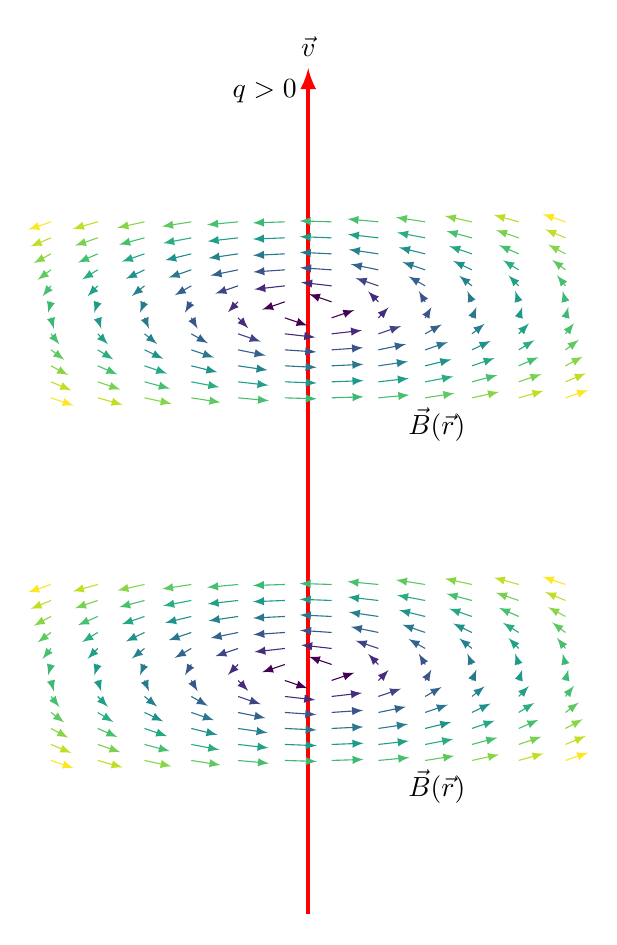
\begin{tikzpicture}
\begin{axis}[
  xmin = -2, xmax = 2,
  ymin = -2, ymax = 2,
  zmin = 0, zmax = 1,
  axis equal image,
  height=7cm,
  view = {90}{20},
  colormap/viridis,
  xtick={\empty},
  ytick={\empty},
  hide axis,
  samples = 12,
  clip=false,
  ]
  \draw[->,red,ultra thick] (axis cs: 0,0,-2) -- (axis cs: 0,0,5) node[above,black] {$\vec{v}$} node[below left,black] {$q>0$};
  \node[below] at (axis cs: 2,1,0) {$\vec{B}(\vec{r})$};
  \node[below] at (axis cs: 2,1,3) {$\vec{B}(\vec{r})$};
  \field{0}
  \field{3}
\end{axis}
\end{tikzpicture}
\end{document}
